\clearpage

\section{Граф вычислений}
\subsection{Абстрактная модель}
\label{sec:abstractmodel}
\begin{figure}[ht]
    \centering
    \includegraphics[width=0.8\linewidth]{graph.png}
    \caption{Структура графа}
    \label{fig:graphstructure}
\end{figure}
Граф представляет собой абстракцию, содержащую хранилище вершин графа с которыми работает пользователь в данный момент (Sync Nodes), сохраненные в графе вершины (Owning Nodes) и множество рёбер (Topology).
\begin{itemize}
    \item \textbf{Sync Nodes} -- множество вершин, объекты которых находятся у пользователя, и с которыми пользователь может работать (изменять, добавлять ассоциирующиеся с ними ребра в граф и т.п.).
    \item \textbf{Owning Nodes} -- множество вершин, сохраненных в графе, доступ к которым пользователь не имеет (заполняется при уничтожении вершины, ассоциируемой с графом, или после явного сохранения вершины пользователем).
    \item \textbf{Topology} -- множество рёбер графа.
\end{itemize}
В данный момент фреймворк позволяет пользователю создать вершины следующих типов:
\begin{itemize}
	\item \textbf{Node} -- вершина, содержащая в себе функцию от результатов входящих в неё вершин.
	\item \textbf{InputNode} -- вершина, позволяющая вносить данные в граф из различных хранилищ данных. Также может служить для хранения параметра графа вычислений, изменяющегося во время процесса оптимизации. 
\end{itemize}
\subsection{Описание алгоритма обхода графа}
\label{sec:algtraverse}
Необходимо выделить последовательность множеств вершин (назовем их кластерами), работа с которыми может проводиться независимо внутри множеств. Кроме того вершинам $i$-го кластера требуются данные только от вершин из предыдущих кластеров. Подобное разбиение позволит с легкостью записать граф в виде обычной программы на некотором языке программирования, а так же выполнить часть операций параллельно, эффективно задействуя многоядерные системы. Для выполнения такого разбиения разработан специальный алгоритм. Сначала будет дано описание алгоритма для графа без ориентированных циклов, в котором любая вершина достижима из вершин нулевого кластера, а затем будут даны замечания о работе алгоритма в обходе графов, нарушающих это правило.
\begin{itemize}
	\item \textbf{Входные данные}: Множество вершин графа, разделенное на вектора вершин соответствующих типов, с указанием количества входящих в каждую вершину ребер и множество рёбер графа.
	\item \textbf{Выходные данные}: Последовательность кластеров вершин, обладаюшая следующим свойством. Пусть $(x_1, x_2)$ - произвольное ориентированное ребро в графе. Пусть вершина $x_i$ содержится в кластере с номером $C_i$. Тогда $C_1 < C_2$. Это свойство означает: если кластеры обрабатываются последовательно, начиная с нулевого, то для любой вершины будет верно, что при старте её обработки будут обработаны все входящие в неё вершины, а значит программа сможет работать с их результатами внутри текущей вершины.
	\item \textbf{Алгоритм}: \begin{enumerate}
	    \item В множество вершин первого кластера заносятся все входные вершины графа. Их кластер назначается текущим.
	    \item Пока из вершин текущего кластера есть выходящие ребра, повторяем:
	    \begin{enumerate}
		\item Создаём новый пустой кластер.
	        \item Проходим по всем ребрам, выходящим из вершин текущего кластера и инкрементируем счетчик вхождений в иные вершины. Если счётчик вхождений в вершину достигает числа входящих в вершину рёбер - вершина добавляется в новый кластер.
	    \end{enumerate}
	        \item Назначаем новый кластер текущим и добавляем в последовательность. В случае если набрался лишь пустой кластер - новый кластер в последовательность не добавляем.
	\end{enumerate}
\end{itemize}
\textbf{Доказательство корректности}: Докажем корректность алгоритма методом математической индукции при условиях, описанных выше.
\begin{itemize}
	\item \textbf{База индукции}: На нулевом шаге формируем нулевой кластер из всех входных вершин. Этот кластер сформирован корректно, т.к. между входными вершинами в графе нельзя строить ориентированные пути.
	\item \textbf{Шаг индукции}: Пусть на $i$-ом шаге корректно сформирован $i$-ый кластер. Начнем формировать $i+1$-ый кластер. Для этого назначим текущим кластером пустой кластер и, проходя по всем выходящим из $i$-ого кластера рёбрам, будем добавлять вершины-концы этих рёбер в текущий кластер. Добавление такой вершины будет происходить тогда, когда она будет посещена в процессе работы алгоритма число раз, равное числу входящих в неё рёбер. Каждое ребро графа в процессе работы алгоритма будет пройдено только один раз, т.к. алгоритм единожды обходит все исходящие рёбра из каждой вершины, а исходить конкретное ребро может лишь из одной вершины. Обход исходящих рёбер для каждой вершины графа будет произведён единожды, т.к. в графе нет ориентированных циклов, а в процессе работы алгоритма переходы в вершины могут осуществляться только в порядке, заданном ориентированными рёбрами графа. Следовательно чтобы добавить вершину в кластер, нужно пройти по всем входящим в неё рёбрам, т.е. вершины, входящие в данную, должны быть добавлены в некоторые из предыдущих кластеров. Таким образом корректность формирования $i+1$-ого кластера доказана.
\end{itemize}
\textbf{Замечание}: Данный алгоритм также позволяет проверить граф на ацикличность и на достижимость произвольной вершины из вершин нулевого кластера. \newline
\textbf{Решение}: Во время обхода графа считать число вершин, добавленных в кластеры.
\begin{itemize}
	\item \textbf{Наличие ориентированных циклов}: Ориентированные циклы могут состоять только из вершин, которые могут иметь входящие и исходящие рёбра. При встрече алгоритма с вершиной ориентированного цикла он не сможет перейти в неё, т.к. существует ребро, являющееся частью этого цикла, но ещё не пройденное алгоритмом, ведь оно исходит из вершины, прежде которой надо посетить ту, в которую алгоритм пытается посетить в данный момент. Следовательно эта вершина не будет добавлена ни в один из кластеров.
	\item \textbf{Достижимость вершин}: Если до какой либо вершины не существует пути от вершин нулевого кластера то она не будет добавлена ни в один из кластеров, т.к. алгоритм переходит от вершины к вершине только вдоль ориентированных рёбер.
\end{itemize}
\subsection{Программное представление вершин}
\label{sec:softwarepresentationnodes}
\begin{figure}[ht]
    \centering
    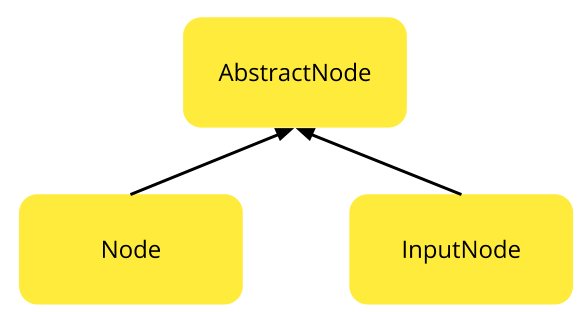
\includegraphics[width=0.8\linewidth]{node_hierarchy.png}
    \caption{Иерархия классов вершин}
    \label{fig:nodes_hierarchy}
\end{figure}
\subsection{Программное представление графа}
\label{sec:softwarepresentationgraph}
Граф представлен классом Graph в пространстве имен athena::core. Основные его поля выполнены следующим образом:
\begin{itemize}
    \item \textbf{Sync Nodes} -- представляет собой объект std::unordered\_set.
    \item \textbf{Owning Nodes} -- представляет собой кортеж векторов, позволяющий содержать объекты всех существующих типов вершин.
    \item \textbf{Topology} -- множество рёбер графа, представленное с помощью std::vector.
\end{itemize}
\subsection{Программное представление алгоритма обхода графа}
\label{sec:softwarepresentationgraph}
\textbf{Входные данные}: 
Множество вершин графа, разделенное на вектора вершин соответствующих типов, с указанием количества входящих в каждую вершину ребер и множество рёбер графа, представленное неотсортированным вектором. \newline
\textbf{Выходные данные}: 
Далее выполняются шаги:
\begin{enumerate}
    \item Отсортировать вектор рёбер. Назначить каждой вершине индекс, показывающий начало подвектора исходящих из неё рёбер.
    \item В множество вершин первого кластера заносятся все входные вершины графа. Их кластер назначается текущим.
    \item Пока из вершин текущего кластера есть выходящие ребра, повторяем:
    \begin{enumerate}
        \item Проходим по всем ребрам, выходящим из вершин текущего кластера и инкрементируем счетчик вхождений в иные вершины.
        \item Все иные вершины, счетчик соответствующий которым сравнялся с числом входящих в них на данной итерации рёбер кладем в новый кластер, назначаем его текущим и добавляем в последовательность. В случае если набрался лишь пустой кластер - новых элементов в последовательность не добавляем.
    \end{enumerate}
\end{enumerate}
